Selles peatükis analüüsime eelmises peatükis kirjeldatud katsete tulemusi, et mõista, kuidas erinevad mudelikonfiguratsioonid ja treeningstrateegiad mõjutavad metsastunud ja lageraielõikude tuvastamise täpsust satelliitpiltidelt. Arutatakse ka tulemuste statistilist olulisust ning võrreldakse erinevate lähenemiste efektiivsust.
\section{Tulemuste võrdlus}
\textbf{Baasjoon}

Eksperimendi käigus testiti süstemaatiliselt erinevaid hüperparameetreid, et leida optimaalne konfiguratsioon antud ülesande jaoks. 
Esitatud tulemuste analüüs näitas, et parimad mudelid
saavutasid märkimisväärselt kõrgeid Dice'i skoore, ulatudes kuni \textasciitilde
0.984. See on eriti üllatav, arvestades andmestiku väiksust.

Parimaks osutunud mudeli konfiguratsioon oli järgmine:
\begin{itemize}
  \item \textbf{Arhitektuur:} Unet
  \item \textbf{Enkooder:} ResNet50
  \item \textbf{Enkooderi kaalud:} ImageNet (eelkoolitatud)
  \item \textbf{Optimeerija:} AdamW
  \item \textbf{Õpisamm:} \textasciitilde 1.09e-4
\end{itemize}

Ka teised kombinatsioonid,
näiteks DeepLabV3 koos ResNet50-ga, saavutasid kõrgeid tulemusi (Dice > 0.97).
Osaliselt on tipptulemused visualiseeritud ka lisatud joonisel \ref{fig:segmentation_results}.

\textbf{Kõrgete skooride põhjused}
Kõrgeid tulemusi väikesel andmestikul võib seletada mitme teguriga.
Siirdõpe (\textit{Transfer Learning}): ImageNet andmestikul eelkoolitatud enkooderite
kasutamine on tõenäoliselt peamine edu võti. Eelnevalt treenitud mudelid omavad
juba võimekust tuvastada üldiseid visuaalseid mustreid (nt servad, tekstuurid),
mida saab efektiivselt kohandada spetsiifilisele metsanduse segmenteerimise
ülesandele. See vähendab oluliselt vajamineva treeningandmestiku mahtu. Peaaegu
kõik parimad tulemused saavutati just imagenet kaaludega. 
Ülesobitamise(\textit{Overfitting}) risk. Kuigi valideerimistulemused on kõrged, tuleb väikese
andmestiku puhul alati arvestada ülesobitamise ohuga. Samas näitab analüüs, et paljudel juhtudel valideerimis- ja treeningkahju
(val\_loss, train\_loss) vähenesid sünkroonis, mis viitab sellele, et mudelid
suutsid siiski valideerimisandmetele edukalt üldistuda ega õppinud
treeningandmeid lihtsalt pähe.

\begin{figure}[H]
    \centering
    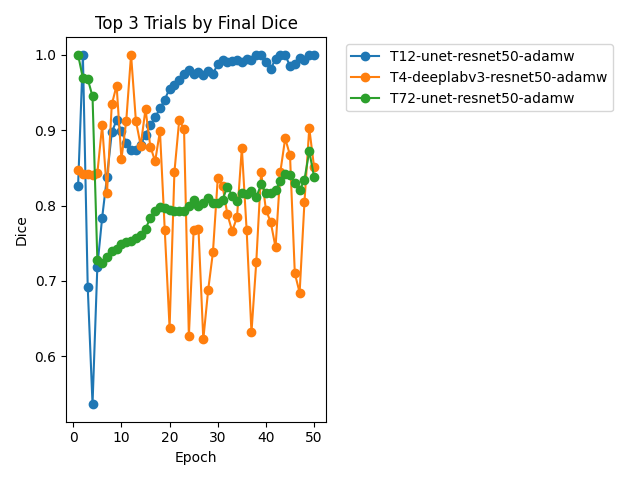
\includegraphics[width=0.8\textwidth]{figures/top3_dice.png}
    \caption{Parimad DICE tulemused erinevate mudelite vahel.}
    \label{fig:segmentation_results}
\end{figure}

Samas individuaalsed klassi tulemused (nt metsastumine vs lageraie) Dice skoorid näitasid suuresti, et mudel ei suuda
täpselt eristada metsastumist ja lageraielõike. Kõrge skoor tuleneb suuresti tagatausta suurest osakaalust pildil. Joonisel \ref{fig:sidebyside_forest_bg} on näha et ülejäänud tausta keskmine Dice skoor on 0.98, mis on väga kõrge. Aga klassipõhised tulemused näitavad, et metsastumise ja lageraielõike eristamine on keeruline. Mudelite katsed ka näitavada, et ka parimate mudelite puhul ei saa nad metsastumist ja lageraielõike eristada.

\begin{figure}[H] % Placement specifier: h-here, t-top, b-bottom
    \centering
    \begin{subfigure}[b]{0.8\textwidth} % Set width for side-by-side arrangement
        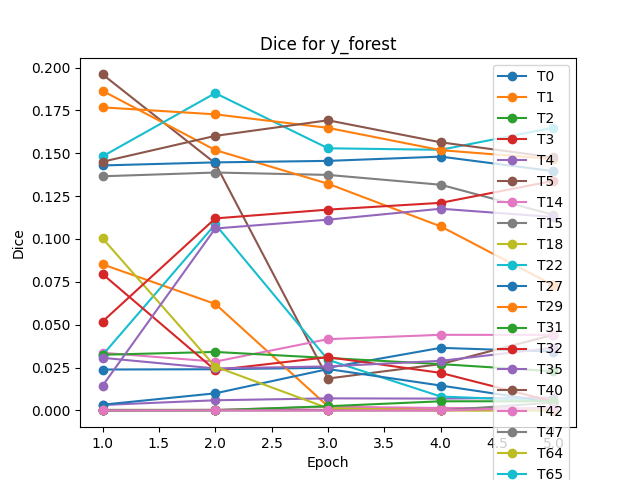
\includegraphics[width=\textwidth]{figures/tulemused/dice_per_class_y_forest.png} % Image path and full width in subfigure
        \caption{} % Leave caption empty to automatically label this subfigure as (a)
        \label{fig:dice_per_class_y_forest}
    \end{subfigure}
    % Second subfigure
    \begin{subfigure}[b]{0.8\textwidth} % Set width for side-by-side arrangement
        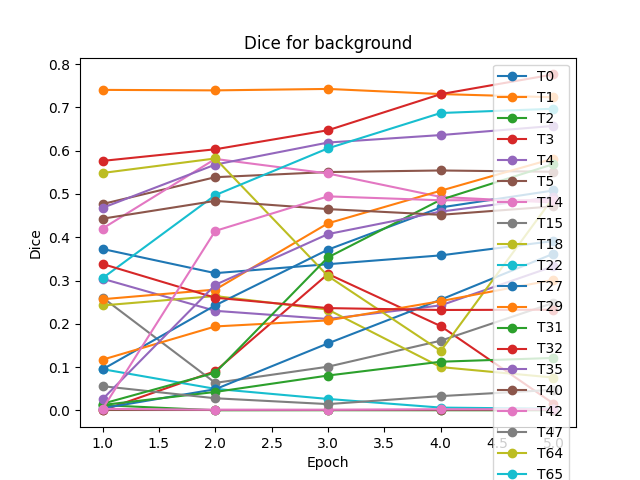
\includegraphics[width=\textwidth]{figures/tulemused/dice_per_class_background.png} % Path and full width in subfigure
        \caption{} % Leave caption empty to automatically label this subfigure as (b)
        \label{fig:dice_per_class_background}
    \end{subfigure}
    
    \caption{Tagatausta ja noore metsa segmentatsiooni Dice tulemused üle katsete} % Main caption for the whole figure environment
    \label{fig:sidebyside_forest_bg} 
\end{figure}




\textbf{Dinov2 eksperimendid}

Käesolevas uurimuses viidi läbi eksperimente, mille eesmärk oli hinnata DINOv2
raamistikul põhinevate masinõppemudelite efektiivsust satelliidipiltide
segmenteerimisel metsanduslikus kontekstis. Katsetati erinevaid Vision
Transformer (ViT) arhitektuure (nt ViT-B/14, ViT-G/14, ViT-L/14, ViT-S/14) koos
erinevate segmenteerimispeadega (nt LinearHead, SimpleHead, FPNHead,
UPerNetHead). Mudelite jõudlust hinnati keskmise Dice'i koefitsiendi, keskmise
IoU (Intersection over Union) ja keskmise täpsuse (Mean Accuracy) alusel,
jälgides neid mõõdikuid kuni 800 epohhi vältel. Treeningutingimustes varieeriti
hüperparameetreid, nagu õppimismäär (nt 1e-5, 5e-5, 1e-4), partii suurus (1, 2,
4) ning rakendati nii külmutamist (Freeze) kui ka peenhäälestamist (FineTune).
\bigskip
\begin{longtable}{llll}
    \textbf{Konfiguratsioon} & \textbf{Mean Dice} & \textbf{Mean IoU} & \textbf{Mean Täpsus} \\
    \hline
    ViTB14 LinearHead LR5e-5 BS2 E5 Freeze & 0.18 & 0.16 & 0.26 \\
    ViTB14 SimpleHead LR1e-5 BS4 E5 FineTune & 0.200 & 0.26 & 0.35 \\
    ViTG14 FPNHead LR1e-5 BS4 E5 FineTune & 0.258 & 0.28 & 0.33 \\
    ViTG14 SimpleHead LR1e-4 BS4 E5 Freeze & 0.22 & 0.275 & 0.350 \\
    ViTL14 UPerNetHead LR1e-5 BS1 E3 Freeze & 0.160 & 0.270 & 0.34 \\
    ViTS14 FPNHead LR1e-5 BS4 E5 FineTune & 0.23 & 0.25 & 0.38 \\
    \hline
    \caption{DINOv2 eksperimendi tulemused}
    \label{tab:dinov2_results}
\end{longtable}
\bigskip

Eksperimentide tulemused näitavad, et DINOv2-põhiste mudelite jõudlus satelliidipiltide segmenteerimisel sõltub oluliselt selgroo suurusest, segmenteerimispea keerukusest ja treeningustrateegiast. Suuremad selgrood (nt ViTG14) ja mitme skaala tunnuseid töötlevad pead (nt FPNHead) andsid parimaid tulemusi, saavutades keskmise IoU kuni 0,28 ja täpsuse kuni 0,38. Peenhäälestamine parandas jõudlust võrreldes külmutatud mudelitega, kuid pikaajalistes treeningutes (500–800 epohhi) ilmnes ebastabiilsus, mis viitab ületreenimisele või ebapiisavale regulatsioonile.

Soovitused edasiseks uurimistööks hõlmavad varajase peatamise ja õppimismäära ajakava rakendamist stabiilsuse suurendamiseks, samuti täiendavate arhitektuuride (nt hübriidmudelite) testimist jõudluse lae ületamiseks. Praegused tulemused pakuvad väärtuslikku alust metsanduslike satelliidipiltide segmenteerimise optimeerimiseks.


\section{Edasiarendus ja täiustamine}
\input{chapters/edasiarendus_ja_täiustamine.tex}